\documentclass[14pt]{article}
\usepackage{hyperref}
\usepackage[utf8x]{inputenc}
\usepackage[english,russian]{babel}
\usepackage{cmap}
\usepackage{amsmath}
\usepackage{graphicx}
\graphicspath{ {./q1_img/} }
\usepackage[left=2cm,right=2cm,
    top=2cm,bottom=2cm,bindingoffset=0cm]{geometry}

\title{Билеты по математическому анализу для коллоквиума 14 ноября }
\author{Шишминцев Дмитрий Владимирович}

\begin{document}
    \maketitle
    \tableofcontents
    \newpage
    
    \section{Множества и операции над ними}
        \textsc{(Условно) Множество  }
         - совокупность некоторых объектов определенных по одному признаку. \\
        $ a \in A $ - элемент a принадлежит множеству A \\ 
        $ a \notin A $ - элемент a не принадлежит множеству A \\ 
        $ A \subset B $ - множество A является подмножеством B \\
        \\
        \textsc{Равенство множеств: } Множества равны если каждый элемент множества A является элементом множества B и наоборот \\
        $A = B \Leftrightarrow \begin{cases}
            x \in A \Rightarrow x \in B \\ 
            x \in B \Rightarrow x \in A
        \end{cases}$\\
        \\
        \textsc{Операции над множествами:}
        \begin{itemize}
            \item Пересечение множеств: $ A \cup B = \{ x| x \in A$ и $x \in B \}$ - коммутативно и ассоциативно
            \item Объединение множеств: $ A \cap B = \{ x | x \in A$ или $x \in B \}$ - коммутативно и ассоциативно
            \item Разность множеств: $ A \backslash B = \{ x | x \in A $и$ x \notin B \} $
            \item Симметричная разность: $ A \bigtriangleup B = (A \backslash B) \cap (B \backslash A)$
            \item Декартово произведение множеств: $ A \times B = \{(a; b) | a \in A, b \in B \}$
        \end{itemize}
        
    
    \section{Отображения и функции}
        \textsc{Отображение (функция) } - правило по которому $ \forall x \in A \exists ! y \in B $ \\
        \\
        Варианты функциональных отображений $F : X \rightarrow Y $
        \begin{itemize}
            \item Функция F сюръективна, если $ \forall y \in Y \exists x \in X :y = F(x)$ - каждый элемент множества Y является прообразом хотя бы одного элемента множества X
            \item Функция F инъективна, если $ \forall x \in X \exists y \in Y : y = F(x) $ - разные элементы множества X переводятся в разные элементы множества Y
            \item Функция F биективна, если она сюръективна и инъективна одновременна
        \end{itemize}
        \begin{center}
            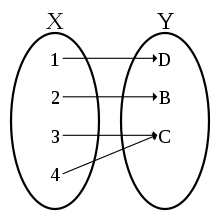
\includegraphics[scale=0.27]{2-1} 
            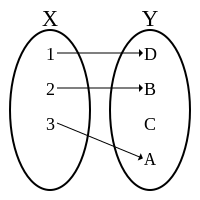
\includegraphics[scale=0.3]{2-2}
            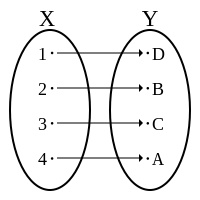
\includegraphics[scale=0.3]{2-3}    
        \end{center}
        
    \section{Эквивалентность, счетность, мощность континума}    
        \textsc{Мощность множества: } $|A|$ - число элементов входящих в множество A \\   
        \textsc{Эквивалентность множеств:} множества эквивалентны $(A \sim B)$ если $|A| = |B|$ \\
        \textsc{Счетность множество: } бесконечное множество, элементы которого можно пронумеровать натуральными числами \\
        \textsc{Мощность континуума: } мощность множества всех вещественных чисел 
 
\end{document}